
% Revisado por Cristina el día 12/03/2013

\srsfuncion{Establecer organización laboral}
	Esta función permite configurar la organización laboral en lo que corresponde a este producto. Se pueden crear y configurar dos niveles de secciones y puestos de trabajo asociados a estas secciones. Sobre las distribuciones se pueden establecer privilegios de acceso a la aplicación, horarios por defecto, salario por defecto y otras configuraciones semejantes. Estas configuraciones son utilizadas por prácticamente todas las funciones del \software desde el registro de personal a la consulta de inventario.

	\begin{enumerate}
		\item \textit{Prioridad}: alta (metafunción).
		\item \textit{Entradas}\\
			El nombre, descripción y configuraciones iniciales anteriormente reseñadas de cada sección y puesto de trabajo.
			\begin{enumerate}
				\item Los nombre de puestos y secciones están limitados a 50 caracteres y sólo podrán contener caracteres considerados alfanuméricos, en todo caso imprimibles.
				\item Las descripciones constarán de un máximo de 200 bytes de caracteres \gls{UTF8}.
				\item Las configuraciones de acceso a las funciones de la aplicación e instalaciones serán colecciones de valores lógicos.
				\item Las configuraciones numéricas: salario base (número decimal no negativo), número de horas de trabajo semanal (número decimal no negativo)\dots{} serán introducidas como texto (en controles filtrados) y convertidas a su valor numérico.
			\end{enumerate}
		\item \textit{Flujo de operaciones}
			\begin{enumerate}
				\item Se muestra una pantalla con las listas de secciones y de puestos de trabajo.
				\item El personal administrativo puede acceder a las opciones de eliminar, modificar o añadir elementos en cada una de las listas. En estas dos últimas se muestra un formulario emergente donde editar o introducir los datos que correspondan.
				\item Cuando el personal administrativo selecciona una sección hoja (que no tiene secciones de nivel inferior) se muestran los puestos de trabajo existentes en su ámbito en la lista de puestos de trabajo.
			\end{enumerate}
		\item \textit{Respuesta a situaciones no previstas}
			\begin{enumerate}
				\item Si no se puede obtener las configuraciones previas de la base de datos, se informa al usuario del error y se aborta la carga de la pantalla.
				\item Si no se pueden almacenar los cambios en el servidor central, informar al usuario y permitirle guardar registro de los cambios para proceder cuando el funcionamiento quede restablecido.
			\end{enumerate}
		\item \textit{Relación con otras funciones}\\
			Prácticamente todas las funciones hacen uso de esta configuración.
	\end{enumerate}

\begin{figure}[ht]\centering
	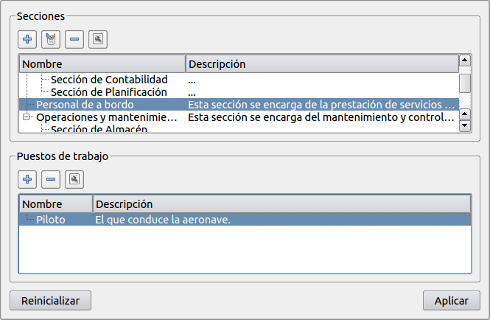
\includegraphics[scale=.6]{imagenes/OrgLaboral.png}
	\caption{Pantalla aproximada del editor de la organización laboral}
\end{figure}
